\chapter{API Contracts Construction with Static Code Analysis}
\label{cha:codeAnalysis}
This chapter explains the concept of constructing caveat contracts from API caveats. In particular, it provides an overview of how caveat sentences from the Java 12 API documentation can be used to construct coding rules similar to code contracts. Applications of static code analysis for these caveat contracts are then explored, with one sample implementation for detecting bugs in real-time described.\bigbreak

\noindent
Section \ref{sec:contract-intro} provides background information for code contracts and an overview of the work conducted for this Chapter: constructing code contracts from API caveat sentences and using static code analysis to apply the contracts to code in real-time. \bigbreak

\noindent
Section \ref{sec:contract-design} describes the design framework for generating and using code contracts. This includes a statistical analysis on the Java 12 API caveats, a description of the idea used for extracting information from caveat sentences for code contracts construction, and the concept of checker programs that can utilise the code contracts. \bigbreak

\noindent
Section \ref{sec:contract-implement} explains the implementation of API contracts construction and static code analysis in an IntelliJ proof-of-concept plugin. \bigbreak

\noindent
Section \ref{sec:contract-results} showcases the IntelliJ plugin developed that uses caveat contracts to detect API misuse. \bigbreak

\section{Introduction}
\label{sec:contract-intro}
Code contracts are a concept derived from object-oriented principles in which preconditions, postconditions, and invariants are defined for different software components. Specifically, the principle of ``design by contract'' suggests the use of specifications for code referred to as contracts. This improves code correctness and robustness as software components can only interact via obligations to code contracts. Using this concept, we can reduce the problem of linking API caveats to source code to the problem of mapping API caveats to code contracts, which we refer to as \textit{API caveat contracts} or simply \textit{caveat contracts} in this thesis. This can be used in real-time to provide feedback during the programming/development process in regards to API caveats. As a continuation of the previous chapter, I perform a statistical analysis of several caveat types for the Java 12 API documentation based on the work by \cite{zhou-directive}. I then propose a parsing technique to construct contracts from API caveats exception sentences, which represent a large proportion of API caveats for the Java 12 API and typically result in exceptions to be thrown. This extends upon the parsing techniques used by both \cite{zhou-directive} and \cite{blasi2018translating} to collect a subset of API caveats related to explicit constraints including \textit{range limitations} or \textit{not-null} constraints. From this, I construct a total of 4,694 unique caveat contracts. Finally, I develop a checker plugin for IntelliJ that uses the caveat contracts to highlight violations of these API contracts in real-time. \\

\section{Design}
\label{sec:contract-design}
The first step to generating contracts for API caveats is the extraction of API caveat sentences. This process was described in the previous chapter (Section \ref{subsec:info-caveat-extract}), and all caveat sentences extracted previously are re-used for this chapter. We recall that caveat extraction for the Java 12 reference documentation yields 
107,601 caveat sentences, where a significant proportion of the sentences are exception sentences or parameter sentences (approximately 30\% and 11\% respectively). These are analogous to the subset of constraints identified and focused in \cite{zhou-directive} and found to represent the largest portion (43.7\%) of API documentation in \cite{directives-study}. From \cite{zhou-directive}, a set of heuristic rules was created from manual inspection that classifies the types of these constraints as (1) nullness not allowed, (2) nullness allowed, (3) type restriction and (4) range limitation. In particular, sentence normalisation techniques were used in both \cite{zhou-directive} and \cite{blasi2018translating} in preparation for parsing techniques. The NLP techniques of POS tagging (identification of part-of-speech categories like nouns for words), dependency parsing (identification of the syntactic structure of sentences) and open information extraction (extraction of relation tuples from plain-text)
are then applied to construct FOL expressions representing the constraints. An SMT solver can then be used to compare whether two FOL expressions are equivalent. This was used in \cite{zhou-directive} by comparing API documentation constraints with the associated code implementations to check whether API documentation was defective. The FOL expressions constructed from code involved traversing the ASTs of programs to extract exceptions thrown and the conditions for those exceptions.\bigbreak

For this thesis, I mainly focus on the \textit{not-null} and \textit{range limitation} constraints identified by \cite{zhou-directive} to reduce the scope of caveat mappings to contracts (given the diversity of API caveats). However, it should be noted that other categories of API caveats could also be transformed with other NLP techniques. Besides this, I base my parsing approach on the sentence normalisation technique used in the previously mentioned work. For static code analysis, I focus on the process used by \cite{zhou-directive} where relevant code elements are first identified, followed by an appropriate analysis of those elements. This can be used by a plugin for some IDE to highlight contract violations (API misuses) while coding. Overall, the design architecture of the approach for this chapter is shown in Figure \ref{fig:contracct-architecture}.

\begin{figure}[h]
	\label{fig:contracct-architecture}
	\centering
	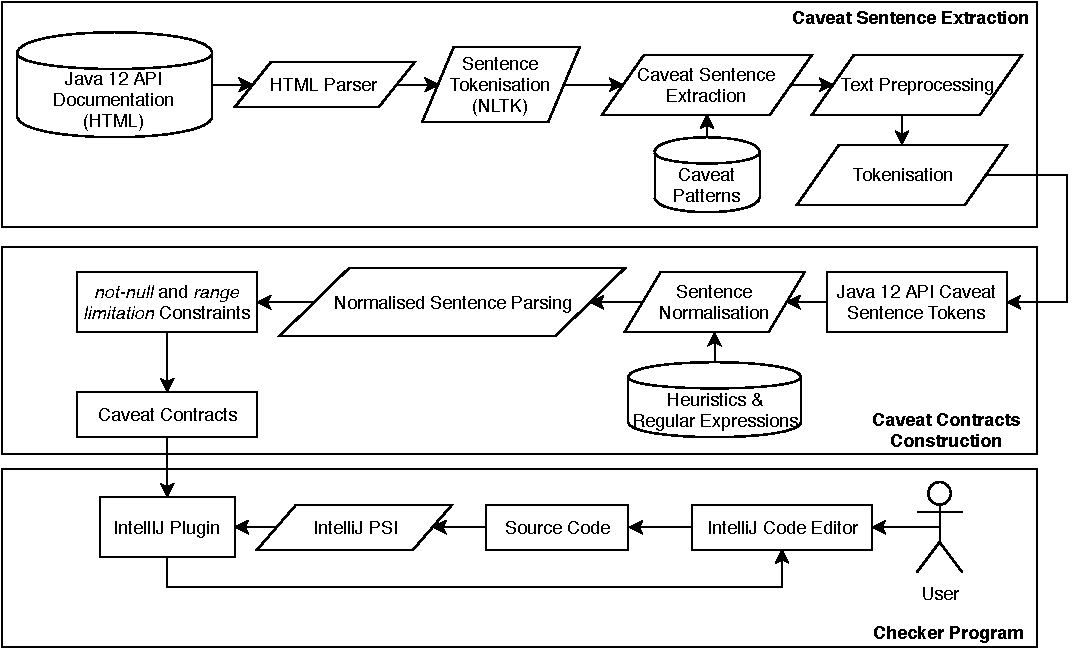
\includegraphics[width=\textwidth]{figs/contract-architecture.pdf}
	\caption{Architecture design of the work for this chapter.}
\end{figure}

Section \ref{subsec:contract-caveat-statistics} provides an overview of the statistical analysis performed for the Java 12 API caveats. This is followed by Section \ref{subsec:contract-construct} that describes the design idea for parsing and extracting constraints from API caveats. Finally, Section \ref{sec:code-checker} gives an overview of ASTs and how checker programs can utilise caveat contracts.

\subsection{Java 12 Caveat Statistics Analysis}
\label{subsec:contract-caveat-statistics}
An important observation on the exception sentences of the Java 12 documentation is they follow a consistent structure. These sentences follow a template of ``\verb|exception - description|'', where \verb|exception| is the exception class thrown and \verb|description| describes conditions required for the exception to be thrown. An example of this is shown in Figure \ref{fig:api-doc-charAt} with the last sentence. It is noted that similar structures are used for other sentences such as the parameter sentences, which follow a template of ``\verb|param - description|'', where \verb|param| is the name of the parameter for a given method/constructor and \verb|description| is the actual sentence describing some information about \verb|param|.  Overall, this information can be used to trivially separate key parts of caveat sentences found within these sections (i.e. the subject and associated description). For parsing constraints, we are only interested in the description parts of exception sentences, as this is where constraints imposed are described. Therefore, only the descriptions of these sentences are used for analysis. Next, I filter the corpus of exception sentences to obtain a unique set. This is because identical descriptions could be mapped to the same caveat contract with slightly different information only in regards to what exception is thrown.  
Hence, I generate a random sample of exception, caveat sentences based on Equation \ref{sample} for a 95\% confidence interval, 5\% error margin and population size of 4915 (unique exception sentences), which gives an estimated sample size of 356. I also collect a random sample for parameter sentences as a comparison of the results by \cite{zhou-directive}. The same confidence interval and error margin was used for this, but with a population size of 2704 to achieve an estimated sample size of 336.\\

\begin{figure}[h]
	\label{fig:api-doc-charAt}
	\centering
	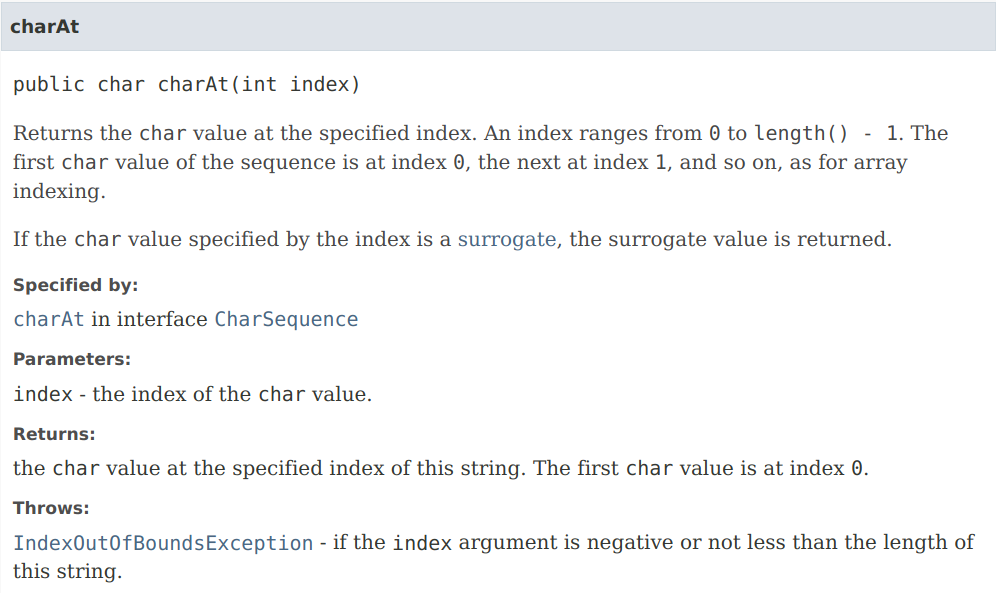
\includegraphics[width=\textwidth]{figs/api-doc-charAt.png}
	\caption{API documentation for the \lstinline{charAt} method of the \lstinline{java.lang.String} class}
\end{figure}

Manual labelling is then required for the samples to identify the prevalence of different caveat types for the sentences. In  particular, the categories identified in \cite{zhou-directive} of \textit{not-null}, \textit{range limitation} and \textit{type restriction} are used as labels with the addition of \textit{ambiguous} to account for sentences that do not match any of the former classes. The \textit{not-null} category involves sentences that specify some parameter cannot be the \lstinline{null} value. The \textit{range limitation} category specifies some limitation involving mathematical logical operators such as a non-negative value requirement (i.e. greater than ro equal to zero). Finally, the \textit{type restriction} category indicates that a parameter must be a particular class type or one of several types. The \textit{nullness allowed} category that was also identified is not considered because it only describes an acceptable condition for contracts, whereas the other categories describe the conditions that constitute an API misuse (or caveat). Overall, the results of this for the parameter sentences sample is shown in Table \ref{tab:caveat-param-stats}, while the results for exception level sentences is shown in Table \ref{tab:caveat-exception-stats}. We note that for \ref{tab:caveat-exception-stats}, the counts add up to more than 356 because 6 of the labelled caveat samples exist in both the \textit{not-null} category and the \textit{range limitation} category. 

\begin{table}[h]
	\centering
	\begin{tabular}{|l|cccc|}
		\hline
		& \multicolumn{4}{c|}{\textbf{Labels}} \\ \cline{2-5} 
		& \textbf{ambiguous} & \textbf{not-null} & \textbf{range limitation} & \textbf{type restriction} \\ \hline
		\textbf{Count} & 291 & 26 & 19 & 0 \\ \hline
	\end{tabular}
	\caption{Manually labelled results for classes of 336 randomly sampled parameter level caveat sentences.}
	\label{tab:caveat-param-stats}
\end{table}

\begin{table}[h]
	\centering
	\begin{tabular}{|l|cccc|}
		\hline
		& \multicolumn{4}{c|}{\textbf{Labels}} \\ \cline{2-5} 
		& \textbf{ambiguous} & \textbf{not-null} & \textbf{range limitation} & \textbf{type restriction} \\ \hline
		\textbf{Count} & 242 & 73 & 46 & 1 \\ \hline
	\end{tabular}
	\caption{Manually labelled results for classes of 356 randomly sampled exception level caveat sentences.}
	\label{tab:caveat-exception-stats}
\end{table}

From Table \ref{tab:caveat-param-stats}, it can be seen that approximately 8\% of unique parameter caveat sentences impose a \textit{not-null} constraint and approximately 6\% of the unique parameter caveat sentences impose a \textit{range limitation} constraint. Despite the small percentage of parameter sentences that fit these categories, it is important to note that they represent an important type of API caveats that can cause software failures from exceptions. Furthermore, these caveat types generally contain explicit constraint descriptions that have little dependencies on other API elements, making them simpler to parse and an adequate baseline for constructing caveat contracts. In contrast, the results from Table \ref{tab:caveat-exception-stats} show that a considerably larger subset (20\%) of unique exception caveat sentences specify a \textit{non-null} constraint. This is also observed for the \textit{range limitation} category with approximately 13\% of sentences labelled. \bigbreak

An analysis of other categories is also conducted to determine what other caveat contracts can be constructed. In particular, the categories identified in \cite{code-examples} are derived from API misuse patterns data-mined from code snippets on Stack Overflow, but can also be mapped into contracts. For example, \textit{missing control constructs} can be represented by a caveat contract that defines the control structure around some API call as a requirement. The same concept can also be applied to \textit{missing or incorrect order of API calls} and \textit{incorrect guard conditions}. For the subcategories of \textit{missing control constructs}, which include \textit{missing exception handling}, \textit{missing if checks} and \textit{missing finally}, we observe that they would all require explicit explanations for usage of these control structures. This is because usage of a control structure such as \lstinline{if} or \lstinline{finally} cannot be inferred without stating those keywords. Furthermore, \textit{incorrect guard conditions} could be considered a superset of the constraints analysed previously in \cite{zhou-directive}, though other categories of this superset would most likely be rare occurrences since they were not identified previously. \bigbreak

For analysis, I focus on \textit{missing control structures} and \textit{missing or incorrect order of API calls} categories. Using a similar approach to before, the estimated sample size required is calculated with Equation \ref{sample} for method, constructor, parameter and return sentences, which are 377, 322, 336 and 353 respectively for the unique sentence population sizes of 22,465, 1,992, 2,704 and 4,426. Exception sentences are not considered as they would all be categorised as descriptions of \textit{missing exception handling} or \textit{incorrect guard conditions}. This emphasises the fact that the exception sentences are an important category of API caveats. 

The labelled results are shown in Table \ref{tab:caveat-sent-stats}. Note that \textit{Control} refers to \textit{missing control structures}, \textit{Temporal} refers to \textit{missing or incorrect order of API calls} and \textit{guard} refers to \textit{incorrect guard conditions}.\\

\begin{table}[h]
	\begin{tabular}{|cc|cccc|}
		\hline
		&  & \multicolumn{4}{c|}{\textbf{Labels}} \\ \cline{3-6} 
		&  & \textbf{Ambiguous} & \textbf{Control} & \textbf{Temporal} & \textbf{Guard} \\ \hline
		\multicolumn{1}{|c|}{\multirow{4}{*}{\textbf{Sentence Location}}} & \textbf{Constructor} & 265 & 21 & 6 & 32 \\ \cline{2-6} 
		\multicolumn{1}{|c|}{} & \textbf{Method} & 360 & 9 & 4 & 5 \\ \cline{2-6} 
		\multicolumn{1}{|c|}{} & \textbf{Parameter} & 257 & 2 & 2 & 75 \\ \cline{2-6} 
		\multicolumn{1}{|c|}{} & \textbf{Return} & 352 & 0 & 1 & 0 \\ \hline
	\end{tabular}
	\caption{Manually labelled categories for caveat sentences found in different locations of the Java 12 API documentation.}
	\label{tab:caveat-sent-stats}
\end{table}

The results in Table \ref{tab:caveat-sent-stats} show the size of \textit{Guard} caveat sentences is significantly larger in parameter sentences and the highest for constructor sentences. Meanwhile, method sentences have roughly equal caveat sentences belonging to the \textit{Control}, \textit{Temporal} or \textit{Guard} categories. Overall, this indicates that perhaps API documents rarely contain API methods that require specific call orders or additional control structures, and caveats related to some guard conditions are the most prevalent. This is an interesting result given that the most prevalent type of API misuse found by \cite{code-examples} for 66,897 Stack Overflow posts was related to \textit{missing control constructs}, followed by \textit{incorrect guard conditions} then \textit{missing or incorrect order of API calls}. This  suggests that the Java 12 API documentation does not contain sufficient information for control structures required for some API caveats.

\subsection{API Contracts Construction}
\label{subsec:contract-construct}
Given the results found from statistical analysis in \ref{subsec:contract-caveat-statistics}, the next step is to collect a set of API caveat sentences and attempt to transform them into caveat contracts. As a baseline study, the API caveats contained within the \textit{not-null} and \textit{range limitation} categories are chosen as they represent a sizeable proportion of exception caveat sentences (see Table \ref{tab:caveat-exception-stats}). 
We note that this allows us to base our solution on the 64 heuristic rules and 29 regular expressions from \cite{zhou-directive} designed for parsing mainly \textit{not-null} and \textit{range limitation} constraints. For reference, the approach in \cite{zhou-directive} required intensive manual analysis to formulate the heuristics. Hence, I attempt to extend upon  approaches with a key observation about English sentences and by utilising sentence normalisation techniques by \cite{blasi2018translating}. This resulted in a much simpler approach for extracting constraints that did not require manual analysis to formulate heuristics. \bigbreak

To design a simpler method for parsing API caveats with a \textit{not-null} constraint, we observe that sentences must mention the term ``null'' to either specify if a \lstinline{null} value is allowed/not allowed in code. Furthermore, given the structural information of the Java 12 API documentation for parameter sentences and exception sentences, extracting additional information such as the subjects of the sentences is simple (as described in Section \ref{subsec:contract-caveat-statistics}). Therefore, dependency parsing and POS tagging is not required. Another observation made based on the heuristics from \cite{zhou-directive} is the prevalence of the subject-verb-object (SVO) ordering for English sentences \cite{dryer200581}. Specifically, English commonly follows SVO ordering despite other possible orderings such as subject-object-verb used in Japanese or subject-verb-object in Mandarin. This structure can be seen from rules 1 and 17 of Table \ref{tab:not-null-heuristic} and all rules shown in Table \ref{tab:range-limit-heuristic}. For rule 20, we observe the use of ``non-null` as a predicative adjective to the subject, which is the only \textit{non-null} heuristic formulated that has ``null'' appearing before the subject. \bigbreak 

The final observation for \textit{not-null} caveats is that whether some API method/constructor's parameter can be null is a boolean condition. In other words, this category of caveats represents the simplest form of a caveat contract as it only needs to specify whether a null value is accepted or not accepted. Given this information, a general approach to identify whether an API caveat is of the \textit{non-null} category is to filter out caveat sentences that do not contain the sub-string ``null''. Next, we assume that API documentation aims to be simplistic and mentions of nullness within certain sentences (i.e. parameter or exception sentences) can be regarded as a \textit{non-null} constraint. This is particularly true for the Java 12 API documentation as exception sentences (for example) describe the conditions required for the relevant exception to be thrown. Hence, any mention of ``null'' could be assumed to indicate a null value will result in an exception. We note however that this assumption does not necessarily hold for other API documentation. \\
\clearpage

\begin{table}[h]
	\centering
	\begin{tabular}{|cc|}
		\hline
		Rule Number & Heuristic \\ \hline
		1 & [something] be/equals null \\
		17 & Value of [something] be/equals null \\
		20 & Non-null [something] \\ \hline
	\end{tabular}
	\caption{Example of 3 of 20 heuristic rules for nullness not allowed from \cite{zhou-directive}. Note that the complete list can be found in the Appendix.}
	\label{tab:not-null-heuristic}
\end{table}

\begin{table}[h]
	\centering
	\begin{tabular}{|cc|}
		\hline
		Rule Number & Heuristic \\ \hline
		1 & [something] >/</= [value] \\
		8 & [something] be {not} negative/positive/false/true \\
		20 & [something1] equals [something2] \\ \hline
	\end{tabular}
	\caption{Example of 3 of 23 heuristic rules for range limitations from \cite{zhou-directive}. Note that the complete list can be found in the Appendix.}
	\label{tab:range-limit-heuristic}
\end{table}

An alternative approach for parsing the \textit{non-null} and \textit{range limitation} API caveats is to utilise sentence normalisation techniques used in \cite{zhou-directive} and \cite{blasi2018translating}. In particular, several regular expressions are identified by \citeauthor{zhou-directive} to perform substitutions within a sentence before dependency parsing. These expressions are used to detect cases such as the names of variables, classes, and mathematical expressions, which are then replaced with a predefined token to facilitate dependency parsing. This process is a form of \textit{sentence normalisation}. However, rather than using a dependency parser, we can simply use heuristic rules based on the structure of SVO in English sentences. For example, a sentence in the exception section of the \lstinline{ArrayBlockingQueue} constructor for class \lstinline{java.util.concurrent.ArrayBlockingQueue<E>} says:

\begin{verbatim}
IllegalArgumentException - if capacity is less than c.size(), or less than 1
\end{verbatim}

If we ignore the exception, and focus on the description text after the hyphen as described in Section \ref{subsec:info-caveat-extract}, we obtain:

\begin{verbatim}
if capacity is less than c.size(), or less than 1
\end{verbatim}

From this, we can then apply sentence normalisation techniques previously mentioned. The rules formulated for this project are shown in \ref{tab:normalisation-regex} and are based on those used by \cite{blasi2018translating}. These rules are used first in the normalisation process. For the given example, the first phase of normalisation results in:

\begin{verbatim}
if capacity is < c.size(), or < 1
\end{verbatim}

\begin{table}[h]
	\begin{tabular}{|l|l|}
		\hline
		\textbf{Regular Expression} & \textbf{Normalisation Form} \\ \hline
		(not? (less|shorter) than)|((greater|larger) than or equal to) & \textgreater{}= \\ \hline
		(not? (greater|larger|longer) than)|((less|shorter) than or equal to) & \textless{}= \\ \hline
		(less|shorter) than & \textless{} \\ \hline
		(greater|larger|longer) than & \textgreater{} \\ \hline
		((is|are)? not negative)|((be)? non-negative) & \textgreater{}=0 \\ \hline
		((is|are)? not positive)|((be)? non-positive) & \textless{}=0 \\ \hline
		(is|are)? negative & \textless{}0 \\ \hline
		(is|are)? positive & \textgreater{}0 \\ \hline
		not equal( to)? & != \\ \hline
		equal to & == \\ \hline
	\end{tabular}
	\caption{Regular expressions used to normalise mathematical phrases.}
	\label{tab:normalisation-regex}
\end{table}

The second phase of sentence normalisation involves the regular expressions shown in Table \ref{tab:zhou-regex} from \cite{zhou-directive}. This allows us to utilise the SVO structure of English to perform a greedy parsing approach. The result of this is:

\begin{verbatim}
if @PARAM1 is @EXPR1, or @EXPR2
\end{verbatim}

Here, ``@PARAM1'' represents ``capacity'', which is the first parameter of the method, and ``@EXPR1'' and ``@EXPR2'' represent the mathematical expressions within the sentence. Finally, we extract the constraints from the sentence by exploiting the linear nature of the SVO structure that allows words to be parsed in sequence (from left to right). First, we tokenise the sentence such that a list of tokens is obtained, then iterate over the list in a single pass. States are saved throughout the iteration process based on the token observed at each step of the iteration. These states contain information such as whether a negating word (e.g. ``not'', ``false'') or expression was encountered, which can be used to reverse expressions in later iteration steps. A simplistic rule for the parsing is to construct a caveat contract whenever an expression token is encountered. The last parameter seen can be used to complete this expression. For the given example, both ``@EXPR1'' and ``@EXPR2'' are therefore completed with ``@PARAM1'' to form the constraints $capacity<c.size()$ and $capacity<1$. We note that for the scope of this project, the rules used to construct these constraints are simplistic and only consider these mathematical constraints alongside logical ``or'' conditions as shown in the example above. However, this is sufficient to map API caveat sentences of the \textit{not null} and \textit{range limitation} categories. Other constraint types such as temporal rules for API calls would require much more complex parsing techniques.

\clearpage
% Please add the following required packages to your document preamble:
% \usepackage{multirow}
\begin{table}[h]
	\centering
	\begin{tabular}{|l|l|l|}
		\hline
		\textbf{Type} & \textbf{Description} & \textbf{Regular Expression} \\ \hline
		\multirow{2}{*}{\shortstack[l]{Specific\\Values}} & 0.0, 0.1f, etc. & \textbackslash{}W(-)?{[}0-9{]}+(,{[}0-9{]}+)*((\textbackslash{}.{[}0-9{]}+)?{[}a-z{]}*)\textbackslash{}W \\ \cline{2-3} 
		& \begin{tabular}[c]{@{}l@{}}Member value \\of objects e.g.\\ Location.x\end{tabular} & \shortstack[l]{\textbackslash{}W(\textasciicircum{}(java\textbackslash{}.|javax\textbackslash{}.|org\textbackslash{}.))?\\({[}A-Za-z\_{]}+\textbackslash{}w+\textbackslash{}.)+{[}a-z\_{]}+{[}a-z0-9\_{]}*\\{[}\textasciicircum{}\textbackslash{}.A-Za-z0-9\_{]}} \\ \hline
		\multirow{4}{*}{\shortstack[l]{Class\\methods\\and\\static\\members}} & \begin{tabular}[c]{@{}l@{}}Class methods, e.g.,\\ ClassA.func(Param1)\end{tabular} & \shortstack[l]{\textbackslash{}W{[}A-Za-z\_{]}+{[}A-Za-z\_0-9{]}*\\(\textbackslash{}.{[}A-Za-z\_{]}+{[}A-Za-z\_0-9{]})*\\(\#{[}A-Za-z\_{]}+{[}A-Za-z\_0-9{]}*)?([\textasciicircum()]*)\textbackslash{}W} \\ \cline{2-3} 
		& \shortstack[l]{Static member, e.g. \\ Desktop.Action\#OPEN} & \shortstack[l]{\textbackslash{}W({[}A-Za-z\_{]}+{[}A-Za-z\_0-9{]}*(\textbackslash{}.{[}A-Za-z\_{]}+\\{[}A-Za-z\_0-9{]})*)?(\#{[}A-Za-z\_{]}+\\{[}A-Za-z\_0-9{]}*){[}\textasciicircum{}A-Za-z0-9\_(){]}} \\ \cline{2-3} 
		& All upper case & \textbackslash{}W(\textbackslash{}w+\textbackslash{}.)*({[}A-Z{]}+\_)*{[}A-Z{]}+\textbackslash{}W \\ \cline{2-3} 
		& Class name & \shortstack[l]{\textbackslash{}W({[}A-Za-z\_{]}+\textbackslash{}w+\textbackslash{}.)*{[}A-Za-z\_{]}*{[}A-Z{]}+\\\textbackslash{}w+{[}\textasciicircum{}\textbackslash{}.A-Za-z0-9\_{]}} \\ \hline
		\multirow{11}{*}{Expressions} & A - B & \textbackslash{}W\textbackslash{}w+((\textbackslash{}s+-)|(-\textbackslash{}s+)|(\textbackslash{}s+-\textbackslash{}s+))\textbackslash{}w+\textbackslash{}W \\ \cline{2-3} 
		& A + B & \textbackslash{}W\textbackslash{}w+\textbackslash{}s*\textbackslash{}+\textbackslash{}s*\textbackslash{}w+\textbackslash{}W \\ \cline{2-3} 
		& A * B & \textbackslash{}W\textbackslash{}w+\textbackslash{}s*\textbackslash{}*\textbackslash{}s*\textbackslash{}w+\textbackslash{}W \\ \cline{2-3} 
		& A..B & \textbackslash{}W(?\textbackslash{}s*\textbackslash{}w+\textbackslash{}s*)?\textbackslash{}s*\textbackslash{}.\textbackslash{}s*\textbackslash{}.\textbackslash{}s*(?\textbackslash{}s*\textbackslash{}w+\textbackslash{}s*)?\textbackslash{}W \\ \cline{2-3} 
		& {[}A, B{]} & \textbackslash{}W[\textbackslash{}s*\textbackslash{}w+\textbackslash{}s*,\textbackslash{}s*\textbackslash{}w+\textbackslash{}s*]\textbackslash{}W \\ \cline{2-3} 
		& {[}A..B{]} & \textbackslash{}W[\textbackslash{}s*\textbackslash{}w+\textbackslash{}s*(\textbackslash{}.\textbackslash{}s*\textbackslash{}.\textbackslash{}s*)\textbackslash{}s*\textbackslash{}w+\textbackslash{}s*]\textbackslash{}W \\ \cline{2-3} 
		& A \textless{}\textbackslash{}\textless{}= B \textless{}\textbackslash{}\textless{}= C & \textbackslash{}W\textbackslash{}w+\textbackslash{}s*\&lt;=?\textbackslash{}s*\textbackslash{}w+\textbackslash{}s*\&lt;=?\textbackslash{}s*\textbackslash{}w+\textbackslash{}W \\ \cline{2-3} 
		& A \textgreater{}\textbackslash{}\textgreater{}= B \textgreater{}\textbackslash{}\textgreater{}= C & \textbackslash{}W\textbackslash{}w+\textbackslash{}s*\&gt;=?\textbackslash{}s*\textbackslash{}w+\textbackslash{}s*\&gt;=?\textbackslash{}s*\textbackslash{}w+\textbackslash{}W \\ \cline{2-3} 
		& From A to B & \textbackslash{}W(from\textbackslash{}s+)?\textbackslash{}w+\textbackslash{}s+to\textbackslash{}s+\textbackslash{}w+\textbackslash{}W \\ \cline{2-3} 
		& A != B & \textbackslash{}W\textbackslash{}w+\textbackslash{}s*!=\textbackslash{}s*\textbackslash{}w+\textbackslash{}W \\ \cline{2-3} 
		& \shortstack[l]{Enumeration\\ expression} & \textbackslash{}W (\textbackslash{}s*\textbackslash{}w+\textbackslash{}s*)(,\textbackslash{}s*\textbackslash{}w+\textbackslash{}s*)+,?\textbackslash{}s*or\textbackslash{}s*\textbackslash{}w+\textbackslash{}W \\ \hline
	\end{tabular}
	\caption{The regular expressions identified in \cite{zhou-directive} for sub-sentence substitutions and dependency parsing.}
	\label{tab:zhou-regex}
\end{table}

\subsection{Checker Programs}
\label{sec:code-checker}
The previous section described an approach for constructing caveat constructs. It was implicitly assumed that some program analysis tools existed that could utilise these caveat contracts. Fortunately, such tools do exist and are contained within a field of computer science known as static code analysis \cite{1657940}. Static code analysis uses programs that can perform checks on other programs without executing them. A common data structure used by these tools is Abstract Syntax Trees (ASTs), which models the structure of source code as a tree. Syntactic details of the code are not represented which enable the analysis of code to be significantly simpler. Consider the following code for the Euclidean algorithm:

\clearpage

\begin{verbatim}
while b != 0
    if a > b
        a := a - b
    else
        b := b - a
return a
\end{verbatim}

The AST of the program is shown in \ref{fig:ast}. In particular, ASTs can be used to extract important information such as an API method call, what control structures they reside in, or what parameters are passed to the method. Given a caveat contract, we could then traverse the AST of a program and identify any code expressions and statements that correspond to the relevant API element. Checking if a caveat contract is satisfied then requires one or more of the following processes: observing the surrounding API calls, identifying relevant expressions and statements, inspecting the various control flows of the program, evaluating expressions, and inspecting the API call parameters. \\
The IntelliJ platform was chosen for the development of a proof-of-concept checker given that it was one of the three most popular Java IDEs (next to Netbeans and Eclipse) and provides a simple interface for accessing the AST of Java code. IntelliJ provides an interface known as the Program Structure Interface (PSI) that allows developers to interact with the AST of some program, making the development of a plugin relatively simple.

\clearpage
\begin{figure}
	\label{fig:ast}
	\centering
	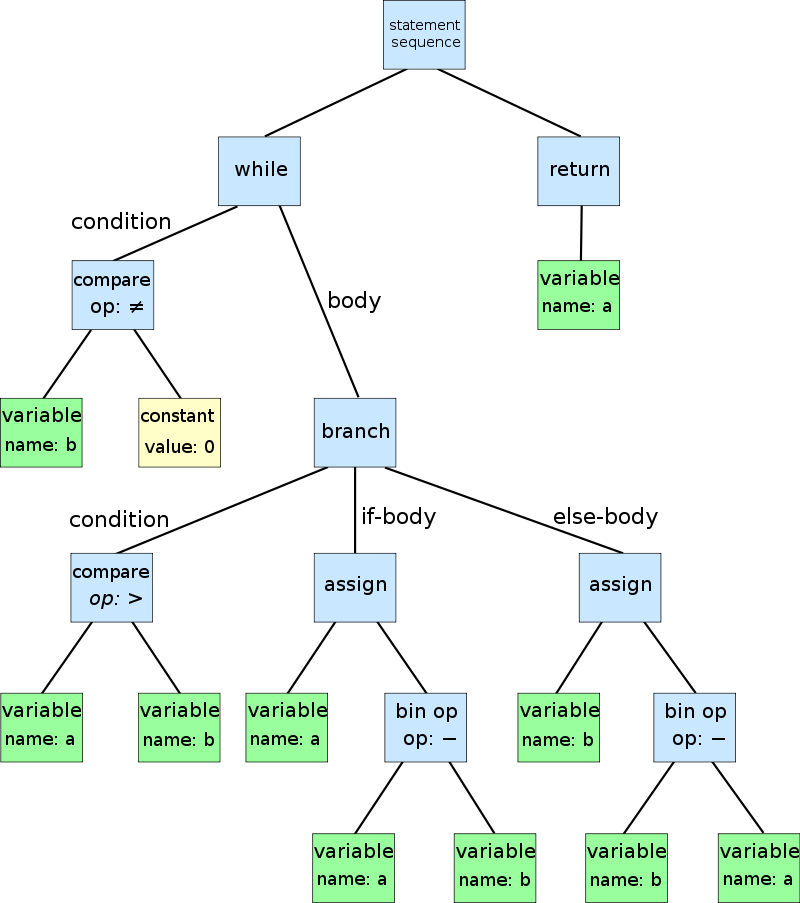
\includegraphics[width=0.75\textwidth]{figs/ast.png}
	\caption{Example of an AST for the Euclidean algorithm. Copied from \url{https://en.wikipedia.org/wiki/Abstract\_syntax\_tree}}
\end{figure}


\section{Implementation}
\label{sec:contract-implement}
Implementation of the caveat contract construction for the Java 12 API was completed using Python 3.6 and its standard libraries. The contracts generated are exported as a JSON array to be used in other applications (i.e. the plugin) and can be found in the project repository of the IntelliJ plugin.

\subsection{Java API Caveat Contracts}
\label{subsec:contract-caveat-contracts}
The caveat sentences extracted from the previous chapter (Section \ref{subsec:info-caveat-extract}) were reused and loaded as a Pandas library\footnote{https://pandas.pydata.org/} \lstinline{DataFrame} object. This object type consists of rows of individual caveats while the columns represent various information about a caveat such as the corresponding caveat sentence and which Java class it belonged to. This allowed filtering functions to be easily applied such that a subset of the caveats could be selected based on certain conditions. Then, constructing the caveat contracts involved following the approach described in \ref{subsec:contract-construct}. In particular, this involves defining the regular expressions from \ref{tab:zhou-regex} and \ref{tab:normalisation-regex} in Python's \lstinline{re} library syntax. A preprocessing step is then performed to reduce the set of caveat sentences that are clearly not \textit{not null} or \textit{range limitation} caveats. For this, I created generalised regular expressions used to identify caveat sentences from these categories based on the fact that likely contained key terms. An example of this is sentences of the \textit{range limitation} category likely contain soon mathematical logical operators such as ``<'' or the text ``less than''. The regular expressions used can be found in Tables \ref{tab:except-null}, \ref{tab:param-null}, \ref{tab:except-range} and \ref{tab:param-range}. Applying these filters reduces the set of invalid caveat sentences and the amount of work required for manually labelling during evaluation.

\begin{table}[h]
	\centering
	\begin{tabular}{|l|}
		\hline
		\textbf{Regular Expression} \\ \hline
		null \\ \hline
	\end{tabular}
	\caption{Regular expressions for identifying exception sentences of the \textit{not-null} category.}
	\label{tab:except-null}
\end{table}

\begin{table}[h]
	\centering
	\begin{tabular}{|l|}
		\hline
		\textbf{Regular Expression} \\ \hline
		not( be)? null \\ \hline
		non-null \\ \hline
	\end{tabular}
	\caption{Regular expressions for identifying parameter sentences of the \textit{not-null} category.}
	\label{tab:param-null}
\end{table}

\begin{table}[h]
	\centering
	\begin{tabular}{|l|}
		\hline
		\textbf{Regular Expression} \\ \hline
		\textless{}|\textgreater{}|= \\ \hline
		equal|equal to|equivalent to|illegal value| is (nan|infinite|empty) \\ \hline
		\textbackslash{}b(less|smaller|greater|larger)\textbackslash{}b \\ \hline
		\textbackslash{}b(range|negative|positive|non-negative|non-positive)\textbackslash{}b \\ \hline
	\end{tabular}
	\caption{Regular expressions for identifying exception sentences of the \textit{range limitation} category}
	\label{tab:except-range}
\end{table}
\clearpage
\begin{table}[h]
	\centering
	\begin{tabular}{|l|}
		\hline
		\textbf{Regular Expression} \\ \hline
		\textless{}|\textgreater{}|= \\ \hline
		(less|smaller|greater|larger) than \\ \hline
		negative|positive|non-negative|non-positive \\ \hline
	\end{tabular}
	\caption{Regular expressions for identifying parameter sentences of the \textit{range limitation} category.}
	\label{tab:param-range}
\end{table}


Before the implementation of sentence parsing and contract construction, I perform random sampling for evaluation purposes in later steps. The unique sentences from the \textit{not-null} exception and parameter sentences are identified, totalling 835 and 193 respectively. For the \textit{range limitation} category, the number of unique exception and parameter sentences is 193 and 149. I then randomly generate a sample of size 100 for each of these sets, which is an appropriate sample size given the small sets of unique sentences and for overall simplicity. The relevant parameter for the \textit{not-null} categories of exception and parameter sentences was then identified manually. As an example, for the sentence ``prefix - the prefix of the tag, may not be null'', \textit{prefix} would be marked as the constraint subject. Since the parameter sentences follow a template as described in \ref{subsec:contract-caveat-statistics}, we note that an algorithm to extract the relevant parameter is trivial whereas for an exception sentence like ``if the specified sorted set is null''\footnote{Taken from the constructor of \lstinline{java.util.TreeSet<E>}}, parsing is harder given that the name of the relevant parameter (``s'' in this case) is not used. \bigbreak

Labelling of the \textit{range limitation} sentences was completed by expressing constraints as mathematical expressions. An example of this is with the sentence ``IllegalArgumentException - if iv is null or (iv.length - offset < 2 * (wordSize / 8))''\footnote{ Taken from the \lstinline{RC5ParameterSpec} constructor of the \lstinline{javax.crypto.spec.RC5ParameterSpec} class}, the manually labelled constraint of the sentence would be identified as $iv.length-offset<2*(wordSize/8)$. After labelling, 90\% of the 100 random parameter sentences filtered for \textit{not-null} were found to actually describe a \textit{not-null} constraint. For the exception level sentences, 87\% were found to describe a \textit{not-null} constraint. For the \textit{range-limitation} samples, 49\% and 72\% of the parameter and exception sentences were found to express a \textit{range limitation} constraint, respectively. These results reveal that using basic sub-string searches is viable for identifying \textit{not-null} constraints, but more complex approaches are required for identifying (and extracting) \textit{range limitation} caveats. \bigbreak

For implementing the sentence parsing, we only focus on the exception sentences as a baseline. The sentence normalisation approach is implemented as described in \ref{subsec:contract-construct}, with regular expression from Tables \ref{tab:zhou-regex} and \ref{tab:normalisation-regex} used to perform substitutions with labelled words. The exception sentences are then tokenised by white-space characters and a simple \lstinline{for} loop is used to iterate through the tokens of each sentence. Constraints are then extracted throughout the iteration process whenever incomplete expression tokens are observed. Caveat contracts are then constructed and represented as individual objects that contain the associated class and API element names, alongside the parameter name, constraint operator (such as the ``<'' operator to represent less than) and comparison value. This process results in 4,694 unique caveat contracts. We note that other representations might be required for other caveat categories, but this is sufficient for \textit{not null} and \textit{range limitation} caveats and for use by a checker program. \bigbreak

Manually comparing the caveat contracts constructed and the mathematical expressions from earlier, 41 of the 72 API caveat sentences that contained a range limitation constraint were correctly extracted. Furthermore, the approach was able to extract partially correct constraints for 13 other caveat sentences (where we define partial as part of the complete constraints of the API caveat, but would still cause an exception if not fulfilled). Hence, 54 of the caveat sentences had caveat contracts that could be applied to static code analysis. We note that the approach proposed also collects caveats of the \textit{not null} category by simply using an equality operator (``=='' or ``!=''). Due to this fact, I only focus on caveat constructs using this method and the alternative method proposed using basic keyword searching is not included in Section \ref{subsec:contract-plugin}. \\

\begin{table}[h]
	\centering
	\begin{tabular}{l|l|l|}
		\cline{2-3}
		& \textbf{Predicted Non-constraint} & \textbf{Predicted Constraint} \\ \hline
		\multicolumn{1}{|l|}{\textbf{Actual Non-constraint}} & 25 & 2 \\ \hline
		\multicolumn{1}{|l|}{\textbf{Actual Constraint}} & 19 & 54 \\ \hline
	\end{tabular}
	\caption{Confusion matrix for the sentence normalisation approach proposed.}
	\label{tab:conf-mat}
\end{table}

Overall, the results found are represented in terms of a confusion matrix in \ref{tab:conf-mat} to allow computation of accuracy, precision, recall, and F-measure scores. It can be seen that the true positive (TP) is 54, true negative (TN) is 25, false positive (FN) is 2, and the false negative is 19. Using the equations \ref{accuracy}, \ref{recall}, \ref{precision} and \ref{f-measure}, the accuracy is 0.77, recall is 0.73, precision is 0.96 and F1 score is 0.83. These results suggest that applying a simplistic sentence normalisation is a viable approach for extracting constraints from sentences that describe exceptions thrown under certain conditions. A specific advantage of this approach is that no manual analysis was required (to formulate heuristic rules), and it could easily be applied to other API documentation.

\begin{equation}
\label{accuracy}
\text{accuracy} = \frac{TP + TN}{TP + TN + FP + FN}
\end{equation}

\begin{equation}
\label{recall}
\text{recall}=\frac{TP}{TP + FN}
\end{equation}

\begin{equation}
\label{precision}
\text{precision}=\frac{TP}{TP + FP}
\end{equation}

\begin{equation}
\label{f-measure}
\text{F1}=\frac{2\cdot recall\cdot precision}{recall + precision}
\end{equation}

\subsection{IntelliJ Plugin with Static Code Analysis}
\label{subsec:contract-plugin}
IntelliJ's PSI provides the \lstinline{AbstractBaseJavaLocalInspectionTool} class that can be extended for creating plugins involving static code analysis. This is used to define a \textit{visitor} that traverses the AST of a program periodically. In addition to this, I defined several classes to represent the concepts of an API method, API class, caveat, and for storing a collection of all caveat contracts loaded from \ref{subsec:contract-caveat-contracts}. Java's \lstinline{HashMap} is used as the underlying data structure for storing the caveat contracts. This allows searching for the contracts of an arbitrary method to consist of two simple, efficient steps: obtaining the methods attached to a certain class (via the full class name as a hash) and finding the correct method by searching through the associated list of methods. It is noted that further optimisations could be made in future to quicken the retrieval of contracts for a given API method. An example of this is using the hash of the method signature to map directly to its caveat contracts. However, a simple design was chosen given that the plugin was a proof-of-concept checker. \bigbreak

The code analysis process involves implementing the visit function for the visitor such that each expression call in the program is identified and analysed. Specifically, the full class name, method name and argument types are identified and compared to the set of caveat contracts associated with that API element. Each caveat contract is then invoked and checked against values provided by the AST, such as the argument values provided to the API call. For the \textit{not-null} constraints, this check simply requires comparing the argument values to a \lstinline{null} value. For the \textit{range limitation} constraints, the logical operators ($<$, $\leq$, etc.) are identified from the caveat contracts and mapped to a Java boolean expression involving the included comparison value from specified by the contracts. This meant that an SMT solver was not required and we could simply apply the range constraints within Java code, though it is noted that an SMT solver could be used in for more complex constraints. As a baseline checker program, only argument values passed directly to an API method call are analysed. IntelliJ's PSI then provides the functionality to register a problem that will be displayed within the code editor of the IDE. Each caveat contract that was found to be violated would then result in a problem to be registered for the associated API call.

\section{Results}
\label{sec:contract-results}
The complete process of constructing caveat contracts from some API documentation and applying it to a checker program was described and implemented. To showcase the checker plugin and its functionalities several examples are of constraint violating code is shown in Figure \ref{fig:plugin-inspection-off}. Using the plugin, the result is each constraint-violation is highlighted in IntelliJ with red squiggly lines as shown in Figure \ref{fig:plugin-inspection-on}. Hovering the cursor over any of these highlighted problems will reveal a pop-up that provides more detailed information about the caveat contract violation. An example of this is shown in \ref{fig:plugin-problem}. These examples are shown with IntelliJ version 2018.2.4 (community edition). This could prevent obvious contract violations for developers (in real-time) and clearly highlight the associated API caveats to guide them towards correct API usage.

\begin{figure}[h]
	\label{fig:plugin-inspection-off}
	\centering
	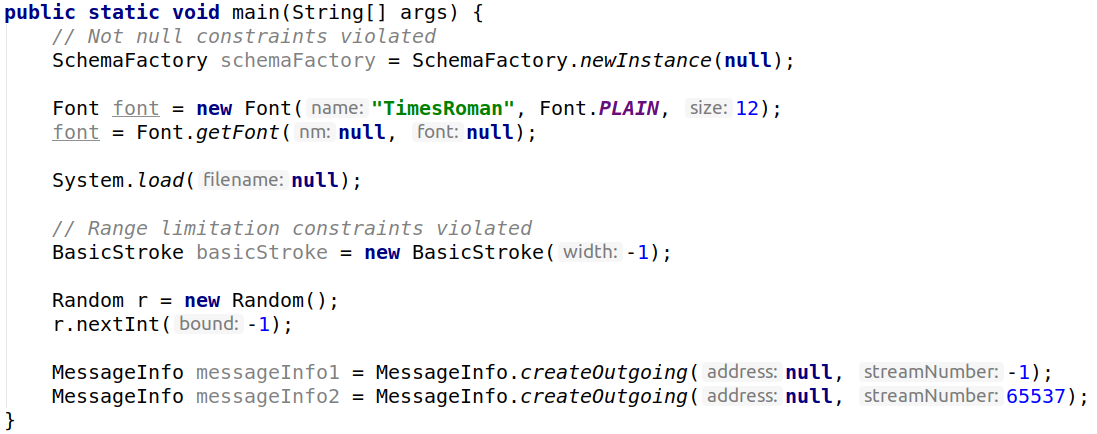
\includegraphics[width=\textwidth]{figs/plugin-inspection-off.png}
	\caption{Example of IntelliJ's (lack of) problem highlights for obvious constraint violations.}
\end{figure}

\begin{figure}[h]
	\label{fig:plugin-inspection-on}
	\centering
	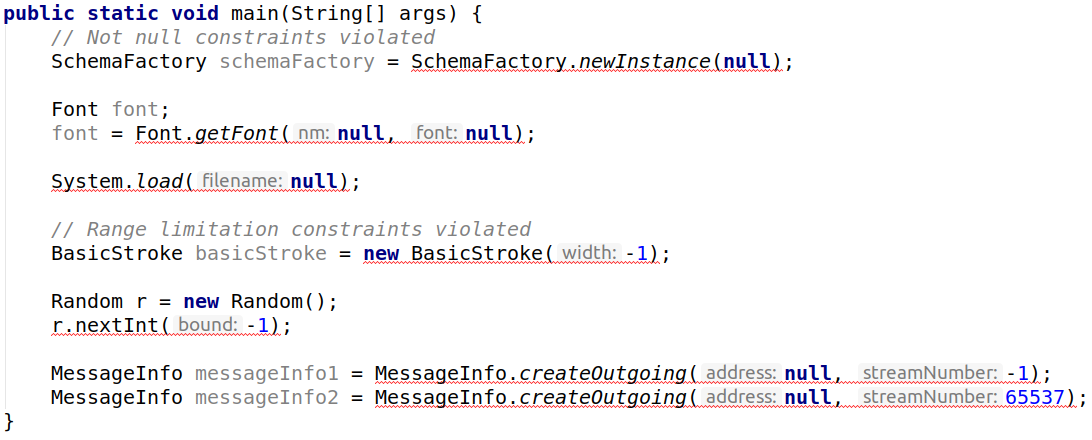
\includegraphics[width=\textwidth]{figs/plugin-inspection-on.png}
	\caption{Example of how the developed plugin handles API caveat contract violations.}
\end{figure}

For interest, it is noted that IntelliJ does implement its version of contracts that require code comment annotations. However, these contracts require special syntax specific to IntelliJ, must be manually implemented for each method and are inconsistent. An example of this inconsistency is shown in Figures \ref{fig:intellij-inspection-on} and \ref{fig:intellij-inspection-off}. In \ref{fig:intellij-inspection-on}, a \textit{not-null} constraint is violated for the \lstinline{isAfter} API call and correctly highlighted by IntelliJ's contracts, but in \ref{fig:intellij-inspection-off} another \textit{not-null} constraint is violated for the \lstinline{add} method of a \lstinline{PriorityQueue} object, which throws a \lstinline{NullPointerException} if executed. Hence, it can be seen that the Intelli's code contracts contain two major drawbacks: it requires the manual implementation of IntelliJ contracts for each method and is prone to errors. The implemented plugin can solve these problems by automating the process of mapping sentences from the Java 12 API documentation to custom caveat contracts. Furthermore, it allows the second problem to be solved with relative ease via manual intervention. This would only involve locating the incorrect caveat contract and modifying it. It can, therefore, be seen that these caveat contracts several improvements and can potentially be extended to other IDEs.

\begin{figure}[h]
	\label{fig:plugin-problem}
	\centering
	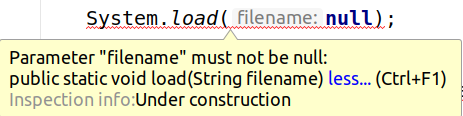
\includegraphics[width=0.6\textwidth]{figs/plugin-problem.png}
	\caption{Example of the displayed problem message for an API caveat contract violation.}
\end{figure}

\begin{figure}[h]
	\label{fig:intellij-inspection-on}
	\centering
	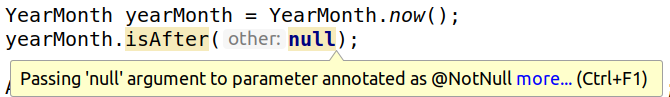
\includegraphics[width=0.7\textwidth]{figs/intellij-inspection-on.png}
	\caption{Example of IntelliJ's contracts.}
\end{figure}

Overall, the plugin in its current iteration is able to highlight the explicit contract violations from the Java 12 API documentation related to \textit{not-null} or \textit{range limitation} constraints. It is clear that with the addition of other categories of API caveats, the plugin could be used to highlight more complex errors and problems for developers in real-time, minimising API misuse and helping developers learn the correct usage of an API. In terms of constructing caveat contracts, further research could yield methods that both improve the precision and recall of constraints extraction. It is noted that only one API documentation was analysed for the scope of this thesis, but the methods proposed apply to other languages and API documentation. \\
One drawback of the plugin is that it can only display warnings after an API misuse, meaning an alternative method is required to teach users about API caveats before a misuse has occurred. This could involve listing potential API caveats from those currently used in a program, though, this is outside the scope of this thesis. In conclusion, the applications of caveat contracts to static code analysis was shown and the idea of mapping natural language to source code to detect API misuse in real-time is plausible, can improve understanding of an API, and potentially increase the efficiency of development by preventing bugs/errors.

\begin{figure}[h]
	\label{fig:intellij-inspection-off}
	\centering
	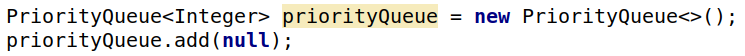
\includegraphics[width=0.8\textwidth]{figs/intellij-inspection-off.png}
	\caption{Example of IntelliJ's contract inconsistency.}
\end{figure}

\section{Summary}
\label{sec:contract-summary}
This chapter focused on the concept of code contracts and how it could be associated with API caveats. The idea of transforming API caveats to contracts was presented and implemented for a subset of API caveats related to \textit{not-null} and \textit{range limitation} constraints. Statistical analysis was also performed to determine the prevalence of these categories of caveats in the Java 12 API documentation. It was found that 20\% of unique API caveat sentences appearing in the exception sections of the documentation imposed a \textit{not-null} constraint. For the \textit{range limitation} category, 13\% of unique API caveat sentences were found to describe a constraint involving range. These categories were chosen for investigation and implementation of code contracts as they provided explicit constraints that result in exceptions. They can also be regarded as the simplest caveats and considered a baseline for mapping natural language to code contracts. Furthermore, an approach for parsing of API caveat sentences to construct caveat contracts was proposed. This was used to extract the not-null and range constraints from sentences, resulting in 4,694 unique caveat contracts. The design and implementation of a proof-of-concept IntelliJ plugin that acted as a checker was also presented. Overall, the potential of this approach for linking natural language to source code was discussed. The plugin showcases that API misuses can be detected in real-time, improve understanding of APIs and direct developers to correct usage of an API.\\
In Chapter \ref{cha:conc}, the findings of this thesis are summarised and ideas for future work are presented.
